\chapter{Progress}\label{progress}
\section{Writing Contributions}

\subsection{Synthetic bed topographies for Antarctica and their utility in ice sheet modelling}
I contributed to the investigation and writing of the manuscript titled "Synthetic bed topographies for Antarctica and their utility in ice sheet modelling," which has been submitted to the journal ``Proceedings of the Royal Society A". This comprehensive review and case study examines the various methods used to generate synthetic bed topographies for Antarctica, assessing their underlying objectives, associated uncertainties, and their impact on ice sheet model projections of sea level rise.

My contribution was focused on the literature review of key methodologies used to generate these topographies. I was responsible for authoring the descriptions for several prominent techniques, including:
\begin{itemize}
\item{Mass Conservation}: Detailing how this physics-informed approach, as implemented in widely-used datasets like BedMachine~\cite{Morlighem_2020} and the TELVIS algorithm~\cite{TELVIS_2011}, is used to reconstruct bed topography by ensuring the continuity of ice volume across the glacial system.

\item{Ensemble Kalman Filter (EnKF)}: Summarising this data assimilation technique which uses an ensemble of model states to estimate and update system parameters based on new observations, thereby tracking the transient evolution of an ice sheet. some relevant works include~\cite{Gillet-Chaulet_2020, Choi_2025}.

\item{Linear Perturbation Theory}: Referenced works using this method are included and discussed in section~\ref{theoretical_frameworks} of this milestone report.

\end{itemize}

By describing these distinct approaches, their physical assumptions, and their limitations, my work helped to establish the theoretical context for the paper's case study on the Aurora Subglacial Basin. This review framed the comparison between different types of synthetic beds ("elevation-preserving" vs. "texture-preserving") and underscored how methodological choices in bed generation can significantly influence projections of future sea level contributions

\newpage
\subsection{SMUG}
I have also contributed to the investigation and writing of a manuscript detailing a new interpolation method for sparse and unevenly sampled data. The manuscript is titled: ``Antarctic bed topography estimation using a Stochastic Meshless Uncertainty Gridding (SMUG) method''. 
% The original conceptualisation of SMUG was developed by Dr. Lenneke Jong, Dr. Jason Roberts and Dr. Felicity McCormack to address the persistent challenges of interpolating Antarctic bedrock topography and robustly propagating the resulting uncertainties.

My contribution involved conducting a review of existing interpolation techniques helping to author the introductory section of the manuscript. My writing establishes the scientific context and rationale for the development of SMUG. I analysed several established methods used in previous Antarctic bed topography datasets, including:

\begin{itemize}
    \item{Inverse Distance Weighting (IDW)}: Used in Bedmap1~\cite{Lythe_2001}, a straightforward method that can produce overly smooth surfaces and struggle with highly variable data.

    \item{Kriging}: A geostatistical method that provides uncertainty estimates but often requires subjective, expert-driven parameter selection, which can introduce bias. This method is evaluated in Bedmap2~\cite{Fretwell_2013} and Bedmap3~\cite{Pritchard_2025} and found to produce less accurate results than other methods such as spline interpolation.

    \item{Spline Interpolation (e.g., Topogrid)}: The key technique in Bedmap2~\cite{Fretwell_2013}, this method demonstrated good performance but faced challenges in optimising smoothing parameters and honouring all data points.

    \item{Mass Conservation Methods}: Implemented in BedMachine~\cite{Morlighem_2020}, this physics-informed approach improves accuracy in data-sparse regions but requires additional datasets (like ice velocity) that are not always available.
\end{itemize}

Through my investigation, I identified and articulated key limitations and research gaps inherent in these widely-used techniques. Specifically, my writing highlighted the common difficulties in providing robust uncertainty estimates, avoiding systematic biases, and capturing the spatial correlation of errors realistically. This analysis sets the stage for the manuscript to introduce SMUG as a method designed to overcome these specific shortcomings, setting the foundation upon which the novelty and significance of the SMUG method were demonstrated in our manuscript. %This manuscript will be submitted TO Elsevier <<<>>>>>

\section{Recreating ISMIP-HOM}

As a first step in validating the computational framework for this project and to build a understanding foundation of the capabilities and functionality of ISSM, I replicated a series of benchmark experiments from the Ice Sheet Model Intercomparison Project for Higher-Order Models (ISMIP-HOM)~\cite{Pattyn_2008}. Successfully replicating these benchmarks demonstrates that the simulation setup is configured accurately capturing the fundamental physics of ice flow.  

Part of my recreation focused on the first four diagnostic experiments (A, B, C, and D), which test a model's ability to simulate ice flow under a range of conditions. Experiments A and B involve flow over a sinusoidally varying bed topography (a "bumpy" 3D bed and a "rippled" 2D bed, respectively) with no basal sliding. These experiments are designed to evaluate the model's handling of longitudinal and vertical stress gradients induced by basal topography. Conversely, Experiments C and D feature a flat bed but introduce spatially variable basal friction, simulating the dynamics of an ice stream with slippery and sticky patches. All my models utilised full-Stokes equations (FS).

\begin{figure}[H]
    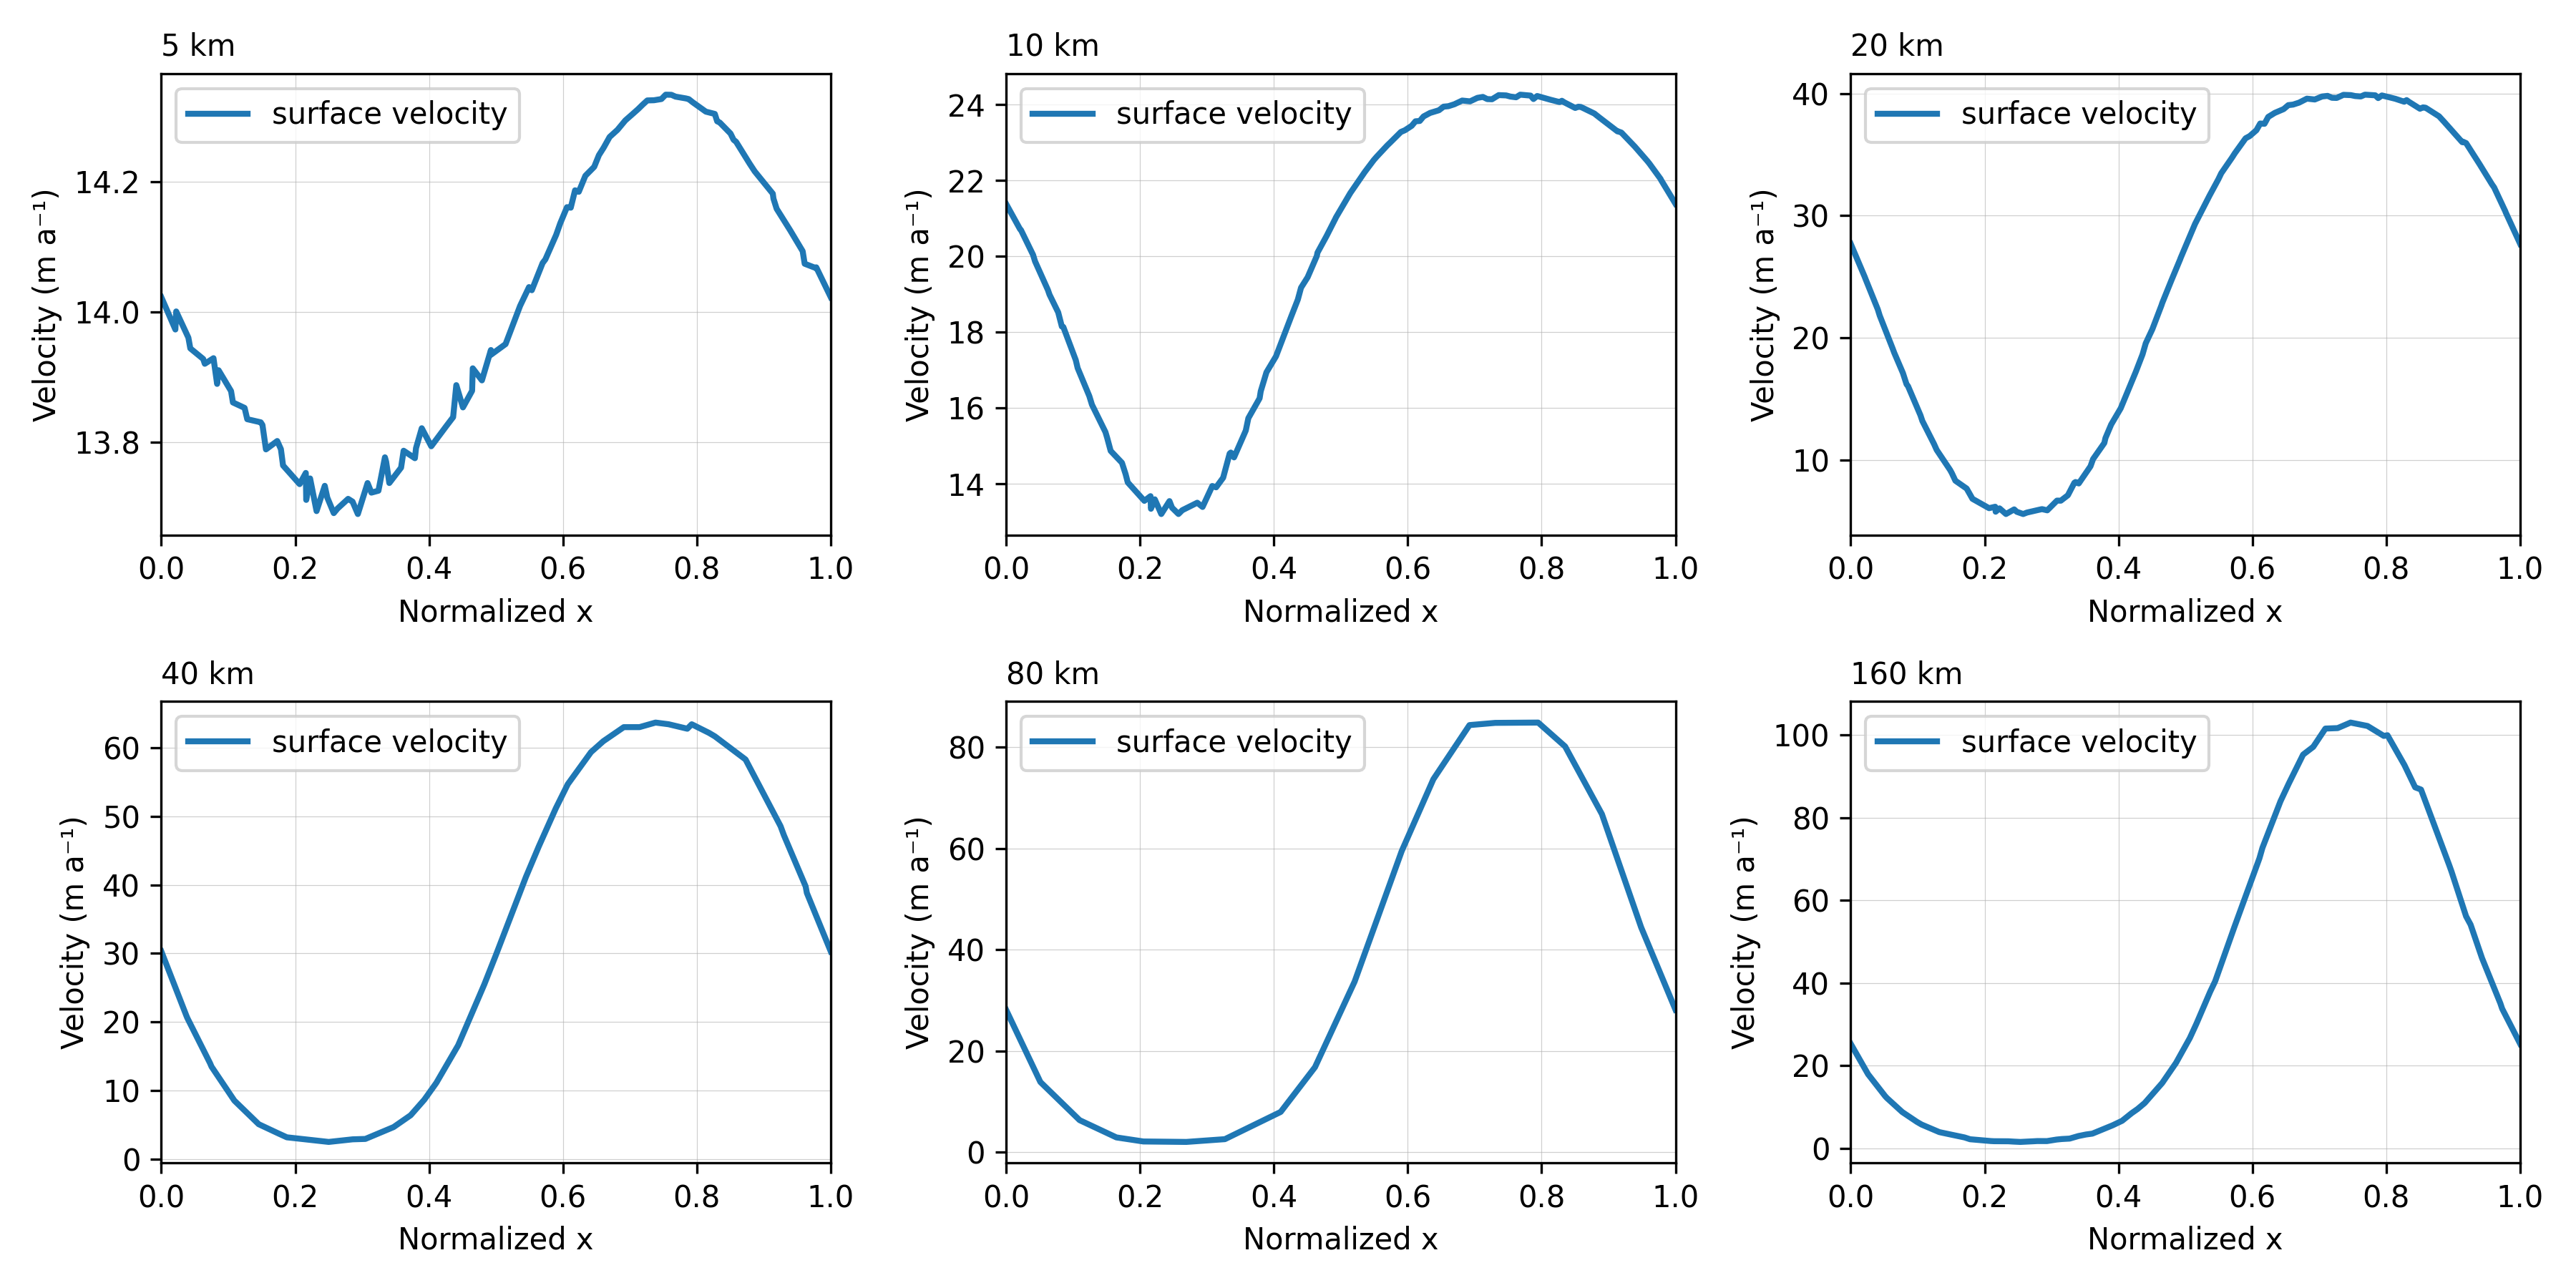
\includegraphics[scale=0.45]{ExpA_velocity_panels.png}
    \caption{ISSM recreation of ISMIP-HOM Experiment A: Ice flow over a bumpy bed. The panels show the the surface velocity for a 3D ice flow simulation over a sinusoidal bed with no basal sliding ($v_b=0$). Each panel corresponds to a different domain length scale (L), from 5 km to 160 km.}
    \label{fig:4.1}
\end{figure}

\begin{figure}[H]
    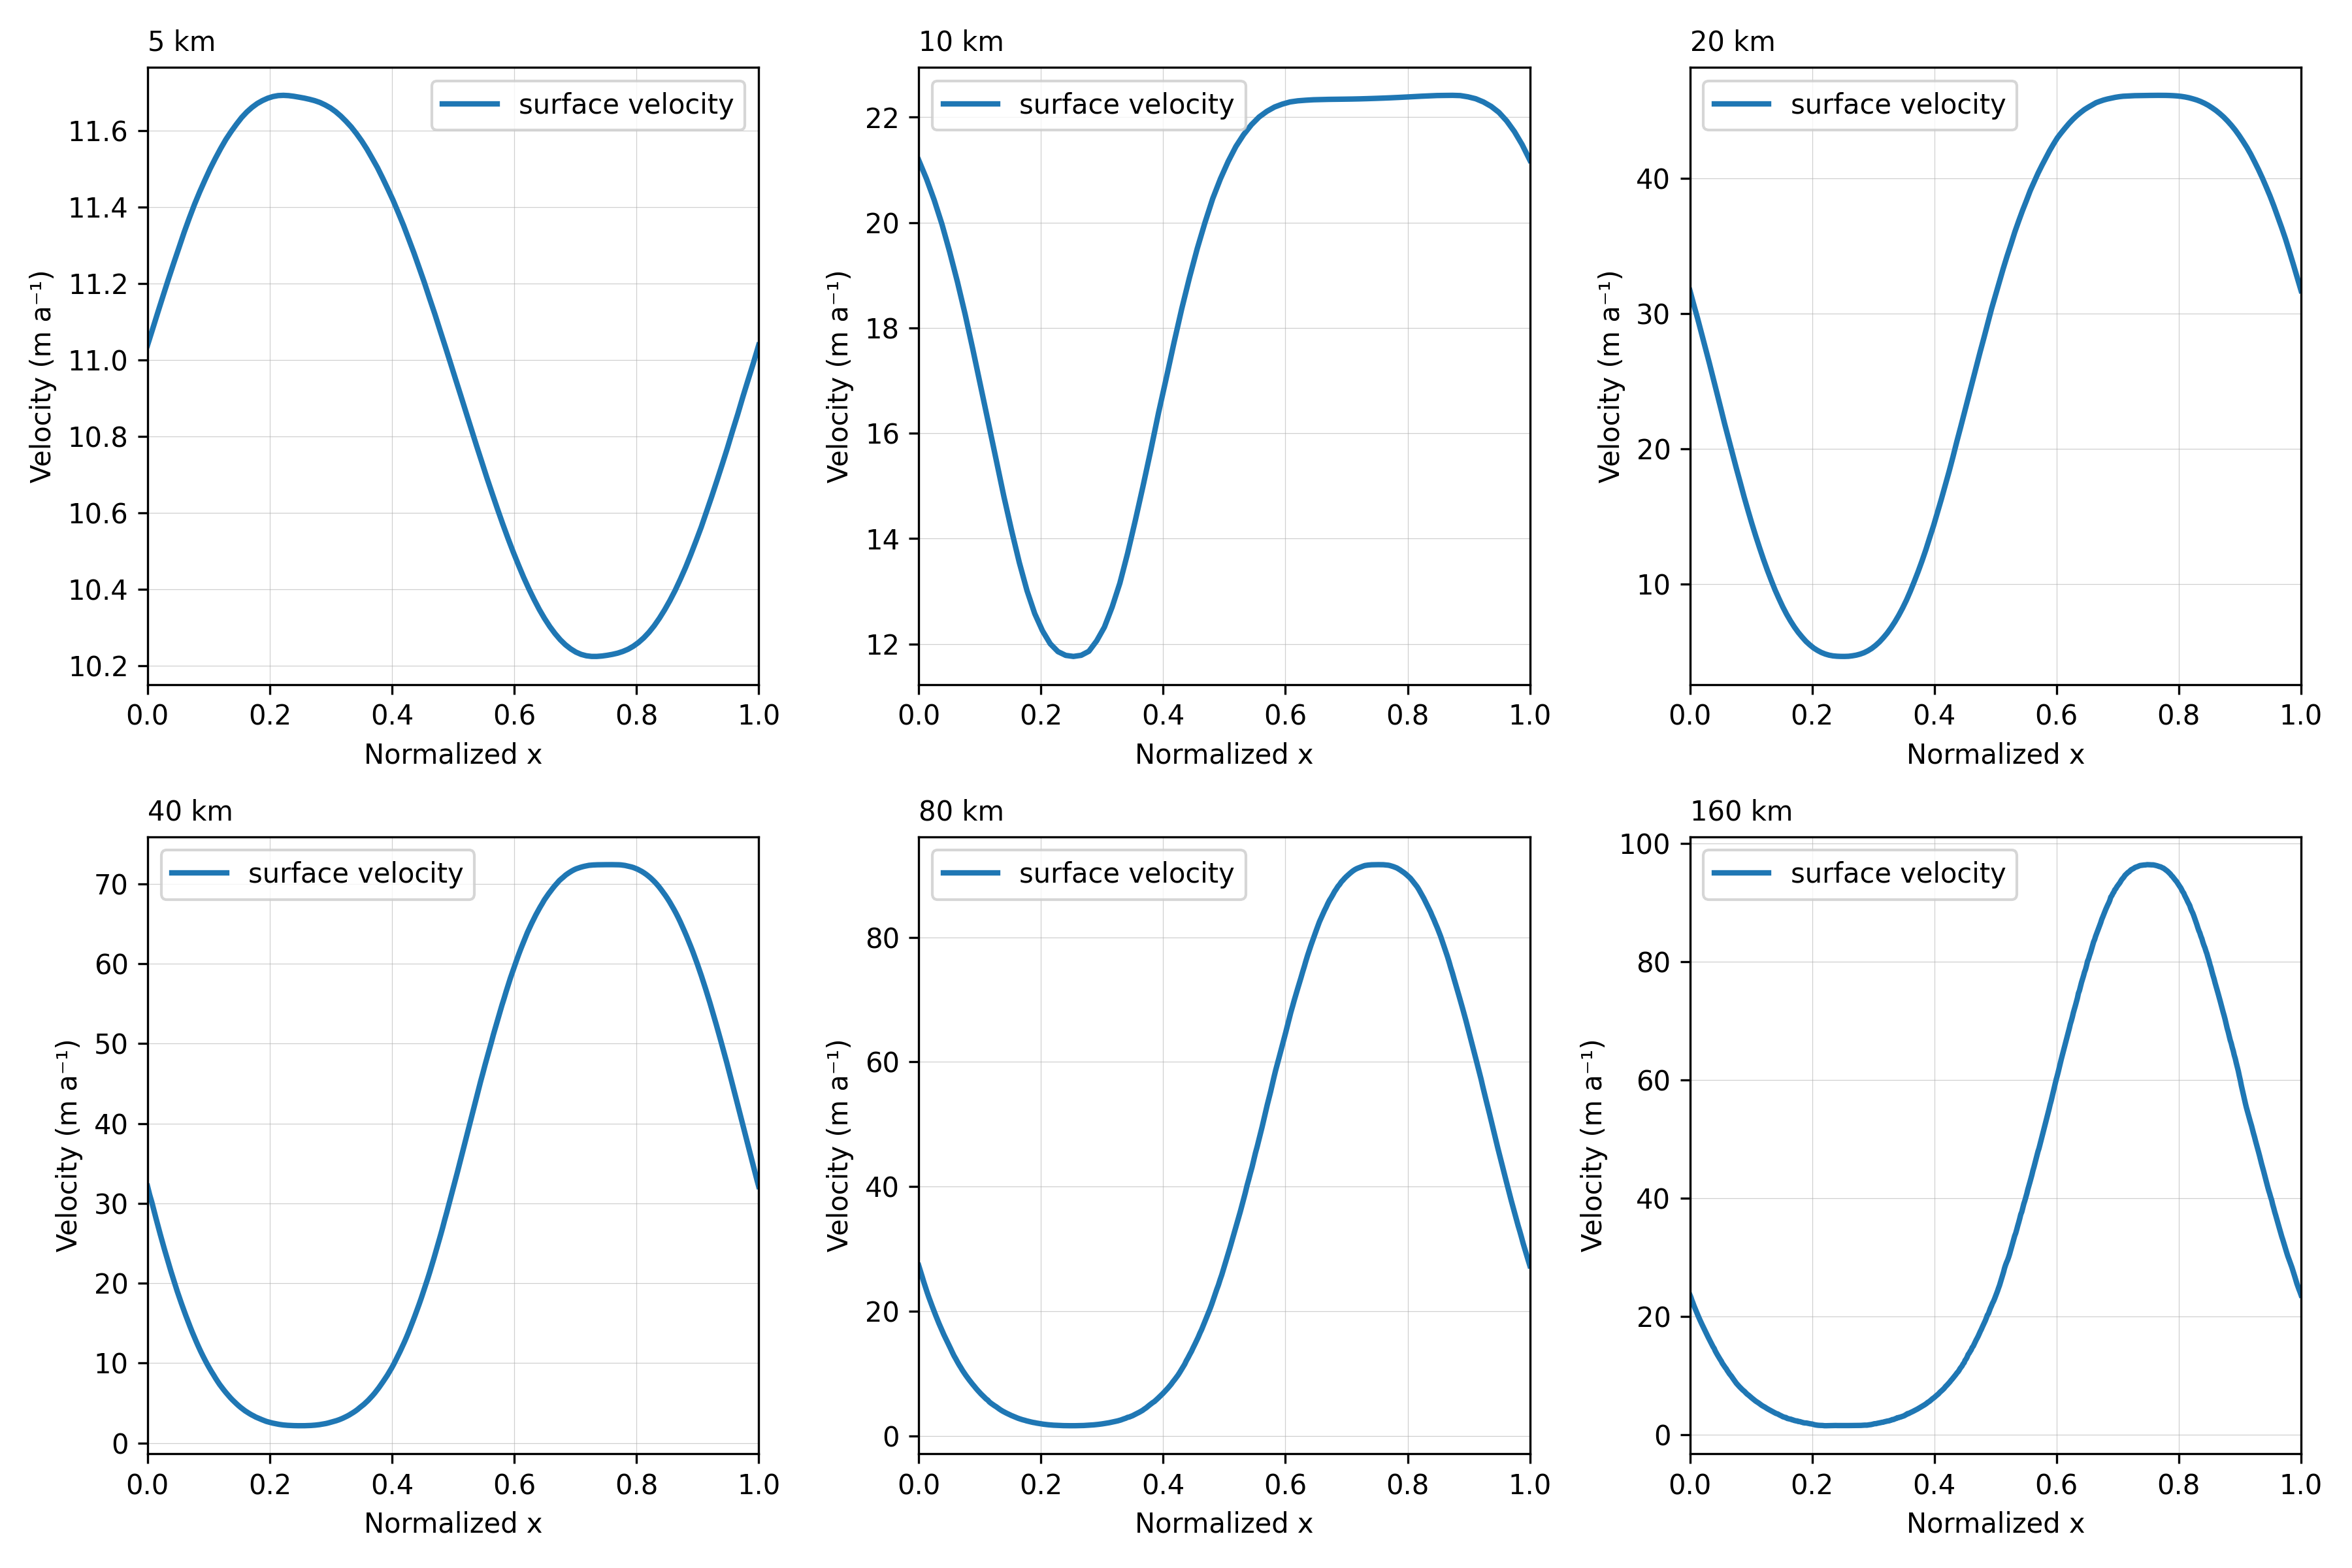
\includegraphics[scale=0.45]{ExpB_velocity_panels.png}
    \caption{ISSM recreation of ISMIP-HOM Experiment B: Ice flow over a rippled bed. The panels show the surface velocity for a 2D flowline simulation. The setup is identical to Experiment A, but the basal topography does not vary in the y-direction, isolating longitudinal stress effects.}
    \label{fig:4.2}
\end{figure}

\begin{figure}[H]
    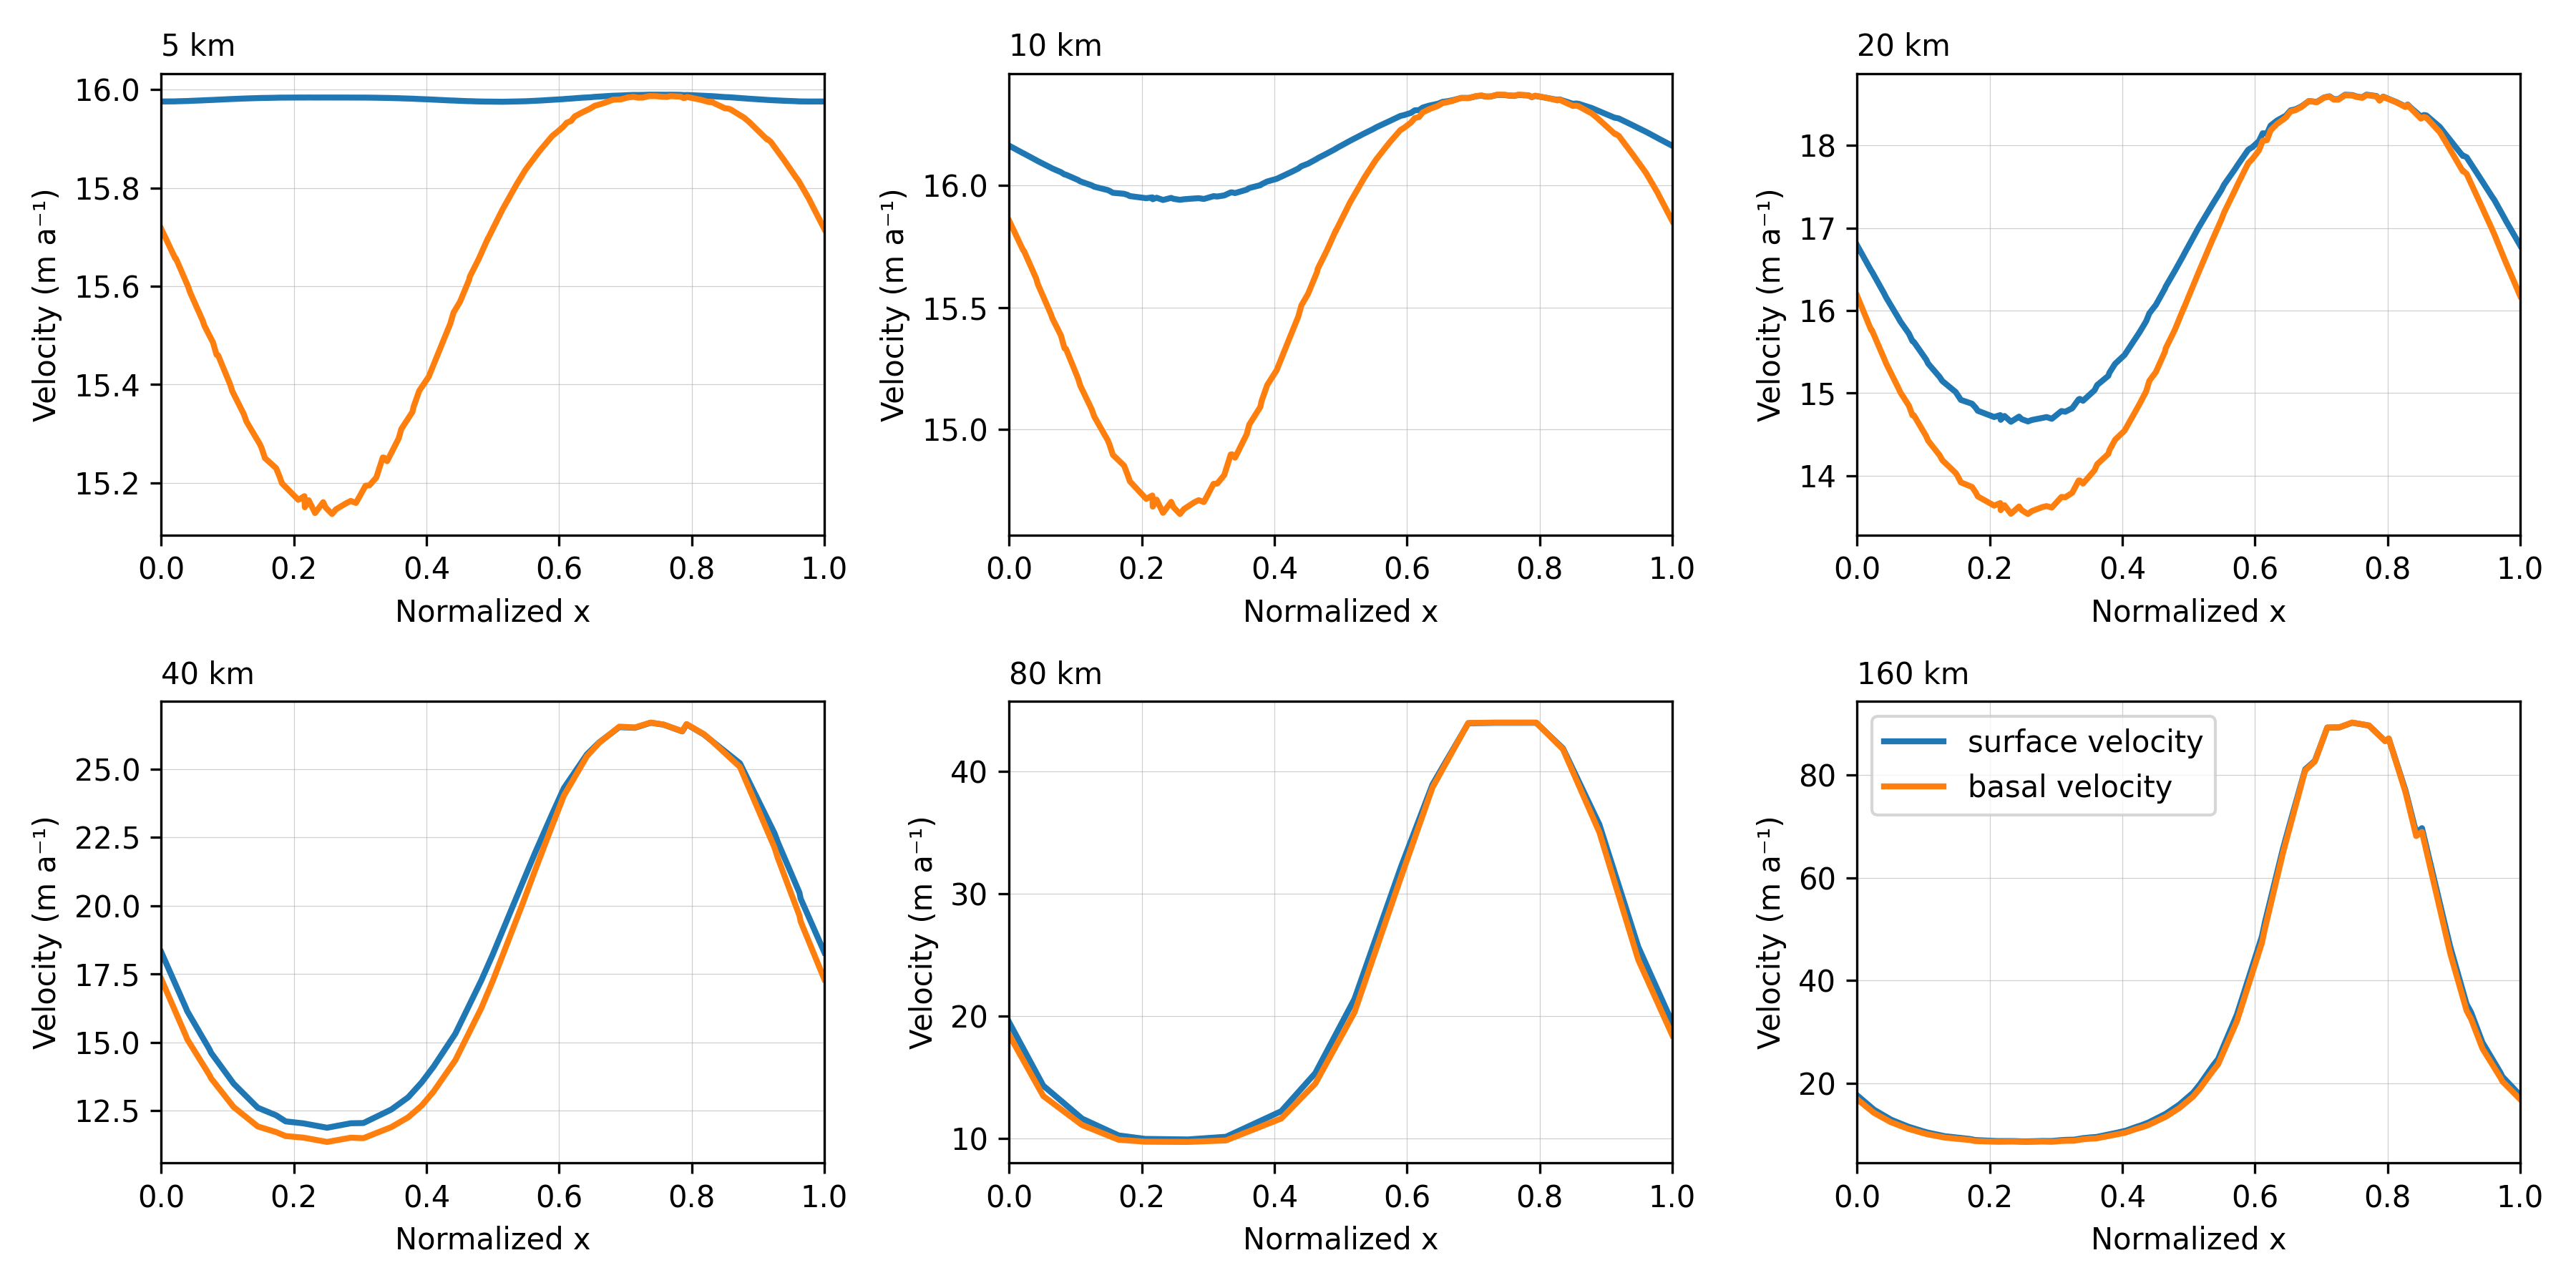
\includegraphics[scale=0.45]{ExpC_velocity_panels.png}
    \caption{ISSM recreation of ISMIP-HOM Experiment C: Ice stream flow I. The panels show both surface (blue) and basal (orange) velocity for a 3D simulation over a flat bed where basal motion is governed by a spatially variable friction coefficient, $\beta^{2}(x,y)$.}
    \label{fig:4.3}
\end{figure}

\begin{figure}[H]
    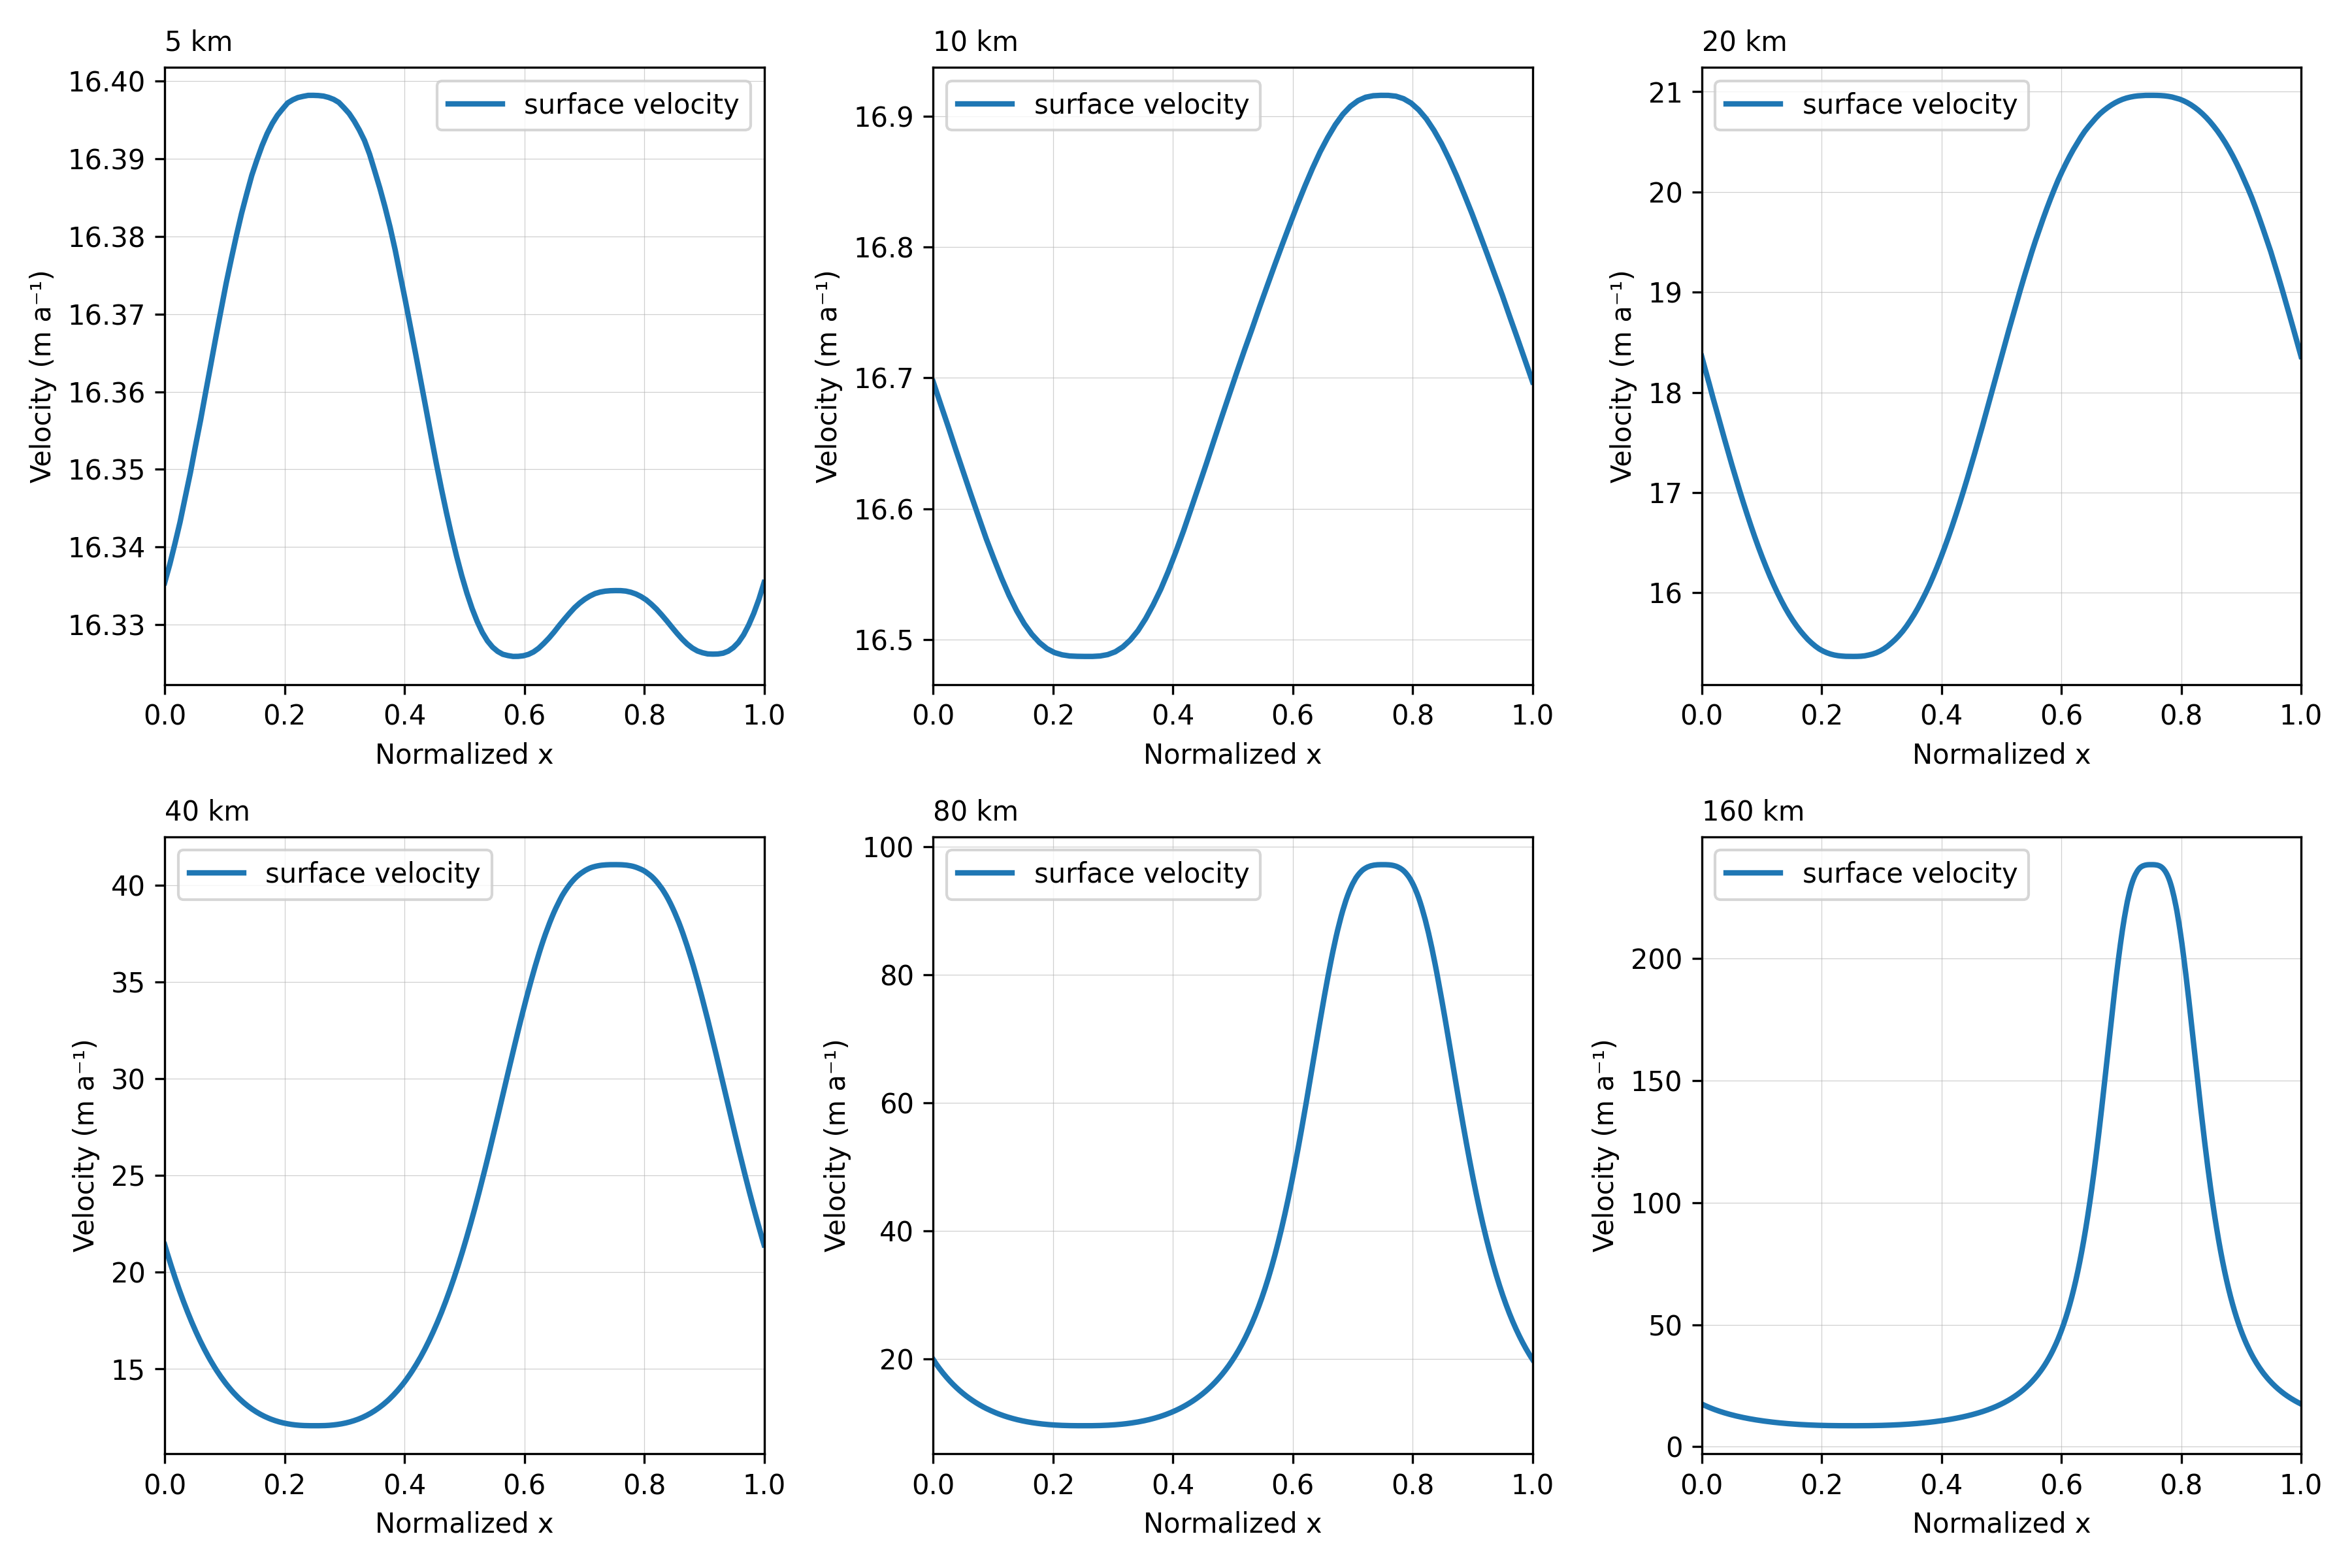
\includegraphics[scale=0.45]{ExpD_velocity_panels.png}
    \caption{ ISSM recreation of ISMIP-HOM Experiment D: Ice stream flow II. The panels show the surface velocity for a 2D flowline over a flat bed with variable basal friction. The setup is identical to Experiment C, but the friction coefficient varies only in the x-direction, $\beta^{2}(x,y)$.}
    \label{fig:4.4}
\end{figure}

The results from these simulations demonstrate a strong agreement with the published findings in~\cite{Pattyn_2008}. For all experiments and across the different prescribed length scales (L = 5 km to 160 km), the calculated surface velocities closely matched the behaviour of the full-Stokes (FS) models from the original ISMIP-HOM. This successful validation confirms that my computational framework is robust and reliably simulates complex ice dynamics. This verification establishes a solid foundation for the application of my framework to more complex simulation settings and its subsequent research questions. In subsection~\ref{transient_ismip} I work on extending the findings in Pattyn et al, 2008. To investigate the transient (Prognostic) experiment F where the free surface is allowed to relax until a steady state is reached for zero surface mass balance~\cite{Pattyn_2008}


\subsection{Transient evolution ISMIP-HOM}\label{transient_ismip}

Building upon the diagnostic ISMIP-HOM experiments, this work extends the prognostic experiment F to systematically investigate the combined effects of rheology and basal sliding within a benchmark ice sheet model. The original experiment F included two scenarios: one with a frozen bed (no-slip) and another with linear sliding. My study expands upon these conditions by also incorporating non-linear rheology. This addition generates four distinct scenarios for comparison:

\begin{itemize}
\item{S1} No-slip (frozen) bed + Linear rheology ($n=1$).
\item{S2} No-slip (frozen) bed + Non-linear rheology ($n=3$).
\item{S3} Linear sliding + Linear rheology ($n=1$).
\item{S4} Linear sliding + Non-linear rheology ($n=3$).
\end{itemize}

While the original study by Pattyn et al. (2008) covered scenarios S1 and S3, understanding the impact of rheological assumptions is crucial for modern ice sheet modelling. During periods of rapid grounding line retreat, uncertainty in the Glen flow law exponent $n$ has been found to cause a larger spread in ice-loss projections than uncertainty in climate forcing~\cite{Getraer_2025}. Therefore, explicitly testing these different physical conditions is a critical step. This foundational analysis, validated against a well-established benchmark, will provide the necessary confidence in the modelling framework before extending the work to a suite of more complex synthetic bed topographies.




In section~\ref{study1}, I extend these principles to investigate the transfer of more complex synthetic bed topography signals to the ice surface. 

\section{Rheology and Sliding Study}\label{study1}

% Budd's sliding theory describes stress propagation through flowing ice over undulating bedrock. The stress field propagates upward at an angle, creating surface (elevation) waves that are phase-shifted by approximately $\pi/2$ relative to bedrock (elevation) features, in Budd's words: \texttt{\texttt{the maximum shear stress occurs at the tops of the waves and the minimum in the troughs''\cite{Budd_1970}}}. 

% As mentioned in section~\ref{paper1}, my work up until now has been focused in building a comprehensive computational framework developed for the systematic investigation of ice dynamics. The first part of this framework is to study via simulations in 2D the ice flowline behavior over a variety of synthetic bedrock topographies to understand the relationship between basal geometry, ice rheology, and overall flow response. A key aim of this work is to understand the effect of commonly made assumptions in ice sheet modelling and their repercussions in the validity of resulting models. This initial stage is designed to be a complete, end-to-end pipeline, from environment setup to final scientific analysis. 

\section{The Computational Framework of this Study}

% This study is supported by a suite of interconnected scripts and tools designed for generating conditions, running simulations, processing output, and performing scientific analysis.

\subsection{Synthetic Bedrock Generation}

% The \texttt{bedrock\_generator.py} script generates synthetic 1D bedrock profiles for ice flow modeling. the core functionality of this script is the creation of realistic bedrock topographies with configurable geometric properties. The bedrock profiles are defined by the following four key parameters that can be varied systematically:
% \begin{itemize}
% \item{Amplitude} Controls the vertical scale of undulations (e.g., 19.2 m to 38.4 m).
% \item{Wavelength} Controls the horizontal scale of undulations (e.g., 3.84 km to 19.2 km).
% \item{Skewness} Controls the asymmetry of the undulations.
% \item{Kurtosis} Controls the peakedness or flatness of the features.
% \end{itemize}

% The generated profiles are saved to \texttt{.npz} files and are loaded by the ice flow simulation script to ensure consistent and reproducible experimental setups.

% \begin{figure}[H]
%     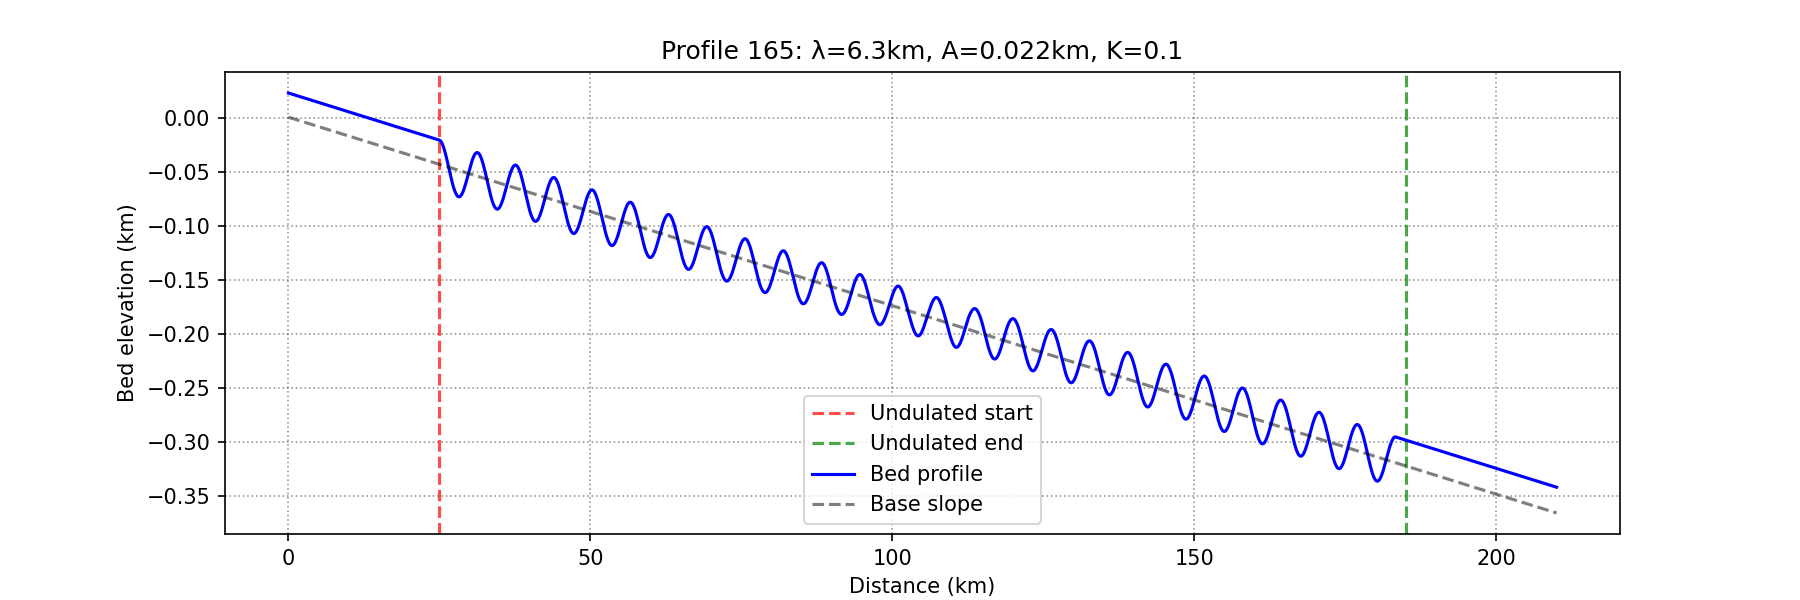
\includegraphics[scale=0.45]{bedrock_profile_165.png}
%     \caption{Database sample: Profile 165 has perturbation wavelength $\lambda=6.336$~km, amplitude $0.022$~km, kurtosis $K=0.1$}
%     \label{fig:}
% \end{figure}
% % def analyse_driving_stress(md, L):
% The domain length for all bedrock profiles is $210$~km with $100$~m horizontal resolution, however the undulated (perturbation) region is $160$~km in length leaving $25$~km flattened areas in the outer regions of the bedrock are there to minimise large driving stress differences between boundaries (something that can be particularly problematic for simulating non-linear rheology scenarios), they also ensure physically consistent periodicity for the numerical simulation.

\subsection{Ice Flow Simulation}

% The core of this study is a time evolution flow simulation of fully grounded ice over 300 years with daily time steps. This simulation is designed to systematically investigate the relationship between basal geometry, ice rheology and flow response by running a series of ISMIP-HOM style experiments~\cite{Pattyn_2008} that can later be analysed in detail with other data processing tools~\ref{dataviz}. The simulations solve the full-Stokes ice flow equations for a static diagnostic stress balance and a transient run (which includes stress balance and mass transport configurations). The simulations utilise the Bidimensional Anisotropic Mesh Generator (BAMG) for the case of 2D flowband meshes (\texttt{bamgflowband}) to create meshes where the mesh resolution is refined based on the underlying bedrock wavelength to capture key physics efficiently. 

% % I have attempted running this simulation in two versions, one is a periodic boundary conditions one and a simple non-periodic flow version

% The simulation utilises periodic boundary conditions which represents a section of an infinitely long flowline, effectively eliminating edge effects that would arise from standard inlet/outlet boundaries. The script couples the inlet and outlet velocities by matching vertices based on their relative depth within the ice column. This ensures that the ice flow is continuous and that the dynamics are driven solely by the underlying topography and internal stresses, which is crucial for studying the transfer of bedrock signals to the surface.
% % =====
% % % This approach proved highly successful, yielding stable and physically realistic velocities (typically < 100 m/a) across all four experimental scenarios. The results are consistent with established benchmarks like ISMIP-HOM and show the expected physical relationships (e.g., faster flow with sliding and non-linear rheology).
% % =====
% % % Technical Note: It is worth noting that while the periodic Full-Stokes model is mathematically well posed,physically robust and runs successfully locally, a technical issue related to a debug assertion in the NCI Gadi supercomputer's ISSM build currently prevents it from running in that specific environment. Investigations confirmed this is a software configuration matter, not a flaw in the model's physics. Consequently, the periodic boundary condition framework is validated as the scientifically superior method for this research.
% % =====

The experimental design is built around four benchmark experiments mentioned in subection~\ref{transient_ismip} to test different physical conditions:

% % Include info on the realism of the setup: Friction, Rigidity, Basal forcings (none implemented)


% % def setup_friction(md, exp):

% % rho_ice = 910 # kg/m^3. From table 1 in Pattyn 2008
% % ice_temperature = (273.15 - 60) # for initialisation <<< MAKE IT COLD AF


% % #>>> CORRECT THIS SHIIIIIIIIII TALK ABOUT THE reference nonlinear and linear work. This 2 script combo is cool

% % # rheology
% % if rheology_n==1:
% %     # if n=1: ISSM interprets the rheology_B parameter as the dynamic viscosity (η)
% %     # in Pattyn for (n=1), the effective viscosity (η) is defined as η=(2A)^−1
% %     A = 2.140373e-7 / yts
% %     rheology_B = (2 * A)**(-1) # = 7.37e13
% % else:
% %     rheology_B = cuffey(ice_temperature)


% % # basal forcing
% % md.basalforcings.floatingice_melting_rate = np.zeros(nv)
% % md.basalforcings.groundedice_melting_rate = np.zeros(nv)

% % # SMB initialisation
% % md.smb.mass_balance = np.zeros(nv)


% % =====

% The main simulation scripts produce \texttt{.nc} files and binary \texttt{.outbin} files for full simulation results (when run locally and on the NCI Gadi system respectively). The \texttt{periodic\_flowline.py} script can also generate text files for quick analysis in the case of the static diagnostic runs.

% % def adaptive_bamg(md, x, s0, b, resolution_factor=1.0):
% The simulation framework in this study includes capabilities for systematic grid convergence testing, comparing solutions across multiple mesh resolutions (e.g., factors of 0.5, 0.75, 1.0, 1.25) to ensure the results are independent of the mesh discretisation, see sections~\ref{grid_ind}.

\subsection{Data Processing and Visualization Tools}\label{dataviz}

% I have developed a set of robust, high-performance scripts to handle the large volume of data produced by the ice flow simulations. (Note that: All these scripts have individual file processing capabilities)

% \begin{enumerate}
% \item{Binary to NetCDF Conversion} A batch-capable tool (\texttt{batch\_convert.py}) converts ISSM \texttt{.outbin} files into the standard, portable NetCDF format. This script supports parallel processing for high throughput.
% \item{Result Extraction and Visualization} A batch script (\texttt{batch\_extract\_results.py}) that automatically finds and processes NetCDF files to generate visualisations of key fields like velocity and pressure. 
% \item{Targeted Scientific Plotting} Additional scripts (\texttt{batch\_plots.py}) are used to create specific scientific plots, such as basal and surface velocities, basal velocity colored over the bed topography and basal shear stress distributions, to analyse the direct impact of the bedrock on flow.
% \end{enumerate}

\subsection{Scientific Analysis Tools}

% \subsubsection{Key Findings: The Grid Independence Study}\label{grid_ind}
% In order to  perform quantitative analysis on the simulation results. I developed a pair of Grid Convergence Analysis scripts capable of analysing the resolution convergence in both the static and transient runs \texttt{analyse\_grid\_convergence.py} and \\\texttt{analyse\_transient\_convergence.py} respectively. Convergence is assessed by comparing solutions from different mesh resolutions (e.g., factors of 0.5, 0.75, 1.0, 1.25) against the finest mesh solution. The primary metric of this script is the L2 relative error, a global, scale-independent measure that quantifies the overall difference between two solutions. An error below $1\%$ is typically considered a sign of good convergence. A standardized $2\times2$ plot~\ref{fig:grid_conv}is generated to provide a comprehensive view of convergence, showing visual velocity comparisons of surface and basal velocities for each mesh resolution tested, numerical L2 error bars, and the computational cost of each resolution.

% %add info on~\ref{fig:transient_conv}

% % \begin{figure}[H]
% %     \includegraphics[scale=0.45]{}
% %     \caption{}
% %     \label{fig:grid_conv}
% % \end{figure}

% % \begin{figure}[H]
% %     \includegraphics[scale=0.45]{}
% %     \caption{}
% %     \label{fig:transient_conv}
% % \end{figure}

% % =====
% % =====
% % My diagnostic convergence analyses show that, for a single test profile (165 in Experiments S1, S2, S3 and S4), coarser resolutions appeared to provide marginally adequate accuracy when compared to the finest resolution factor $0.5$ of the original element size generated by 
% % =====
% % \begin{table}[h]
% % \centering
% % \caption{Corrected Diagnostic Convergence for Profile 022 (Experiment S4)}
% % \begin{tabular}{llll}
% % \toprule
% % Resolution & Surface vx L2 Error & Basal vx L2 Error & Convergence Status \\
% % \midrule
% % 0.75 & 0.41\% & 0.22\% & \textbf{EXCELLENT} \\
% % 1.0 & 0.34\% & 1.30\% & \textbf{MARGINAL} \\
% % 1.25 & 1.17\% & 1.18\% & \textbf{INADEQUATE} \\
% % \bottomrule
% % \end{tabular}
% % \end{table}
% % =====
% % =====

% \subsubsection{Mesh and Transient Fields}
% % # ALSO INCLUDE EXTRANCT RESULTS???

% % THESE ARE ONLY FOR THE CHOSEN FINAL RESOLUTION

% % INITIAL MESH
% % def visual_mesh_check(md):
% % \begin{figure}[H]
% %     \includegraphics[scale=0.45]{}
% %     \caption{}
% %     \label{fig:}
% % \end{figure}

% % FINAL MESH?
% % def visual_mesh_check(md):
% % \begin{figure}[H]
% %     \includegraphics[scale=0.45]{}
% %     \caption{}
% %     \label{fig:}
% % \end{figure}

% % ~~~~~~~~~~~~~~~~~~~~~~~~~~~~~~~~~~~~~~~~~~~~~~~~~~~~~~~~~~~~~~~~~~~~~

% % def plot_transient_fields(md):                                                            
% % \begin{figure}[H]
% %     \includegraphics[scale=0.45]{}
% %     \caption{}
% %     \label{fig:Velocity_magnitude}
% % \end{figure}

% % \begin{figure}[H]
% %     \includegraphics[scale=0.45]{}
% %     \caption{}
% %     \label{fig:Pressure_magnitude}}
% % \end{figure}

% % \begin{figure}[H]
% %     \includegraphics[scale=0.45]{}
% %     \caption{}
% %     \label{fig:base_surface_elevation_magnitude}
% % \end{figure}

% % ~~~~~~~~~~~~~~~~~~~~~~~~~~~~~~~~~~~~~~~~~~~~~~~~~~~~~~~~~~~~~~~~~~~~~

% % def plot_max_velocity_from_netcdf(filename):
% % \begin{figure}[H]
% %     \includegraphics[scale=0.45]{}
% %     \caption{}
% %     \label{fig:}
% % \end{figure}

% % def diagnose_acceleration_onset(md, L)://////////????????
% % \begin{figure}[H]
% %     \includegraphics[scale=0.45]{}
% %     \caption{}
% %     \label{fig:}
% % \end{figure}

% % =====

% % ======================================================

\subsubsection{Phase Analysis}
% To quantify the spatial phase shift between the bedrock topography and the ice surface response and verify the physical validity of my simulation based on the criteria in \cite{Budd_1970}, I developed a single and a batch-processing scripts (\texttt{phase\_analysis.py} and \texttt{batch\_phase\_analysis.py}) that use cross-correlation to calculate the lag and phase shift between the de-trended bed and surface signals for each time step in a given simulation. The scripts generates time-series plots of phase shift evolution and summary text files with numerical results. For each batch or single simulation analysed.

% % \begin{figure}[H]
% %     \includegraphics[scale=0.45]{}
% %     \caption{}
% %     \label{fig:phase_analysis}
% % \end{figure}


% % ======================================================

\subsubsection{Transient Analysis}


% % \begin{figure}[H]
% %     \includegraphics[scale=0.45]{}
% %     \caption{}
% %     \label{fig:Transient_analysis}
% % \end{figure}
